\chapter{\textit{Exokernel}}
O conceito de \textit{exokernel} foi proposto por pesquisadores do MIT na década de 1990. Baseia-se em princípios de \textbf{extensibilidade e minimalismo}. Ele elimina a noção de que o SO deve prover abstrações sobre as quais as aplicações devem ser construídas, ou seja, \textbf{o \textit{kernel} não conhece nenhuma abstração do SO}. Por isso, diz-se que o \textit{exokernel} não oferece uma boa visão global do sistema.

A \textbf{motivação} de tais sistemas é fundamentada no \textit{overhead} inatos aos SO tradicionais, ilustrado na \ref{fig:os-overhead}, os quais tentam prover todas as funcionalidades a todas as aplicações, mesmo que algumas aplicações deixam de usar certas características. Além do \textit{overhead}, estas abstrações escondem informações das aplicações.

\begin{figure}[H]
  \centering
  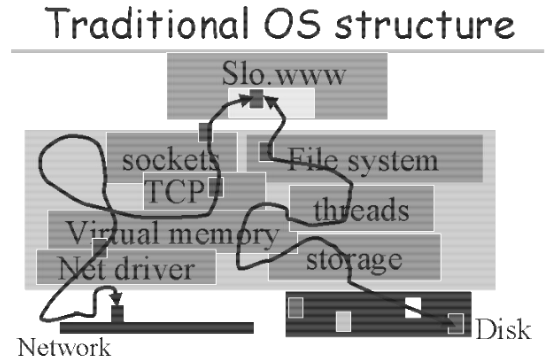
\includegraphics[width=.65\textwidth]{os-overhead}
  \caption{\textit{Overhead} inato de SOs tradicionais}
  \label{fig:os-overhead}
\end{figure}

O \textit{exokernel} concentra-se na multiplexação segura do \textit{hardware}, realizando sua abstração e tornando-o visível às aplicações. De posse das primitivas básicas de \textit{hardware}, podem ser implementadas em modo usuário as abstrações tradicionalmente oferecidas pelo SO.

O \textbf{objetivo} desta abordagem é obter maior \textbf{desempenho e funcionalidade}, já que a aplicação pode customizar o SO de acordo com suas necessidades, o que também acaba provendo \textbf{maior extensibilidade} em relação as arquiteturas monolíticas e de \textit{microkernel}.

Além disso, é garantida uma \textbf{manutenção de código melhor em relação as arquiteturas monolíticas}, uma vez que é mais fácil dar suporte as bibliotecas que implementas estas abstrações.

\section{Arquitetura}
Aqui, o conceito tradicional de um SO é dividido em duas partes:
\begin{itemize}
  \item \textbf{\textit{Exokernel}:} parte que faz a multiplexação segura entre recursos de \textit{hardware}, protegendo os mesmos;

  \item \textbf{LibOS:} conjunto de bibliotecas que gerenciam recursos e oferecem abstrações de alto nível para as aplicações.
\end{itemize}

% TODO: adicionar figura

\subsection{\textit{Exokernel}}
A proteção de recursos de \textit{hardware} feita aqui e \textbf{não se preocupa com a gerência do \textit{hardware}}. Entretanto, o \textit{exokernel} implementa a proteção de memória. Além disso, o \textit{kernel} torna visível:
\begin{itemize}

  \item \textbf{Alocação e Liberação de Recursos:} de posse dos nomes físicos dos componentes de \textit{hardware}, a aplicação pode:
  \begin{itemize}
    \item Alocar recursos através de chamadas de sistema, que verificarão permissões de acesso;

    \item Liberar recursos através de chamadas de sistema;

    \item Verificar o dono do recurso no momento.
  \end{itemize}

  \item \textbf{Nomes físicos do recursos:} com o objetivo de reduzir o número de abstrações e consequentemente aumentar o desempenho, o \textit{exokernel} expõe os nomes físicos do \textit{hardware} e os torna visíveis à aplicação;

  \item Informações sobre a manipulação de recursos.
\end{itemize}


\subsection{Download de Código}
A manipulação de algumas estruturas de \textit{hardware} requer modo protegido, por exemplo, a TLB ou blocos de disco. Por esta razão, o \textit{exokernel} permite que as aplicações descarreguem código no \textit{kernel}, em uma área de memória especial.Esta técnica é chamada de \textbf{\textit{sandboxing}}

Tal técnica garante muito poder a aplicação que descarrega o código, dado que tal código pode extrapolar os limites dessa área de memória, resultando em uma potencial falha de segurança. Entretanto, tal poder pode ser útil para várias aplicações. Isto é uma questão em aberto na literatura.


\subsection{LibOS}
A implementação de abstrações de alto nível é feita pelas bibliotecas LibOSes, \textbf{em modo usuário}, ou seja, não privilegiadas. Isso inclui processos, paginação, arquivos, \textit{drivers}, tratamento de interrupções, memória virtual, mecanismos de IPC e outros. A proteção de memória, no entanto é feita pelo \textit{exokernel}

As LibOSes podem ser criadas ou alteradas pelo usuário. Por isso, elas são \textbf{não confiáveis} (\textit{untrusted}). O usuário também pode elaborar sua própria LibOS, bastando que ele compile e ligue se programa com a biblioteca. Geralmente, são usadas \textit{shared libraries} para tal, o que remove a necessidade de refazer módulos de SO já criados por estas bibliotecas.

Processos utilizam a LibOS, \textit{linkando}-as previamente. Cada processo em execução utiliza o escopo de uma LibOS apenas e uma LibOS pode ser utilizada por vários processos. Nesse caso, é possível que processos de uma mesma LibOS compartilhem recursos abstraídos por ela. Entretanto, processos de diferentes LibOS não podem compartilhar recursos.

\subsubsection{Tratamento de Abstrações Compartilhadas}
Para prover abstrações compartilhadas, o sistema dispõe de alguns mecanismos:

\begin{itemize}
  \item \textbf{Regiões de \textit{Software}:} áreas de memória que só podem ser lidas ou escritas através de chamadas de sistema. Com isso, elas provêm proteção à sub-páginas e isolamento de falhas;

  \item \textbf{Predicados \textit{Wake Up}:} pequenas funções descarregadas no \textit{kernel} que acordam processos quando alguma condição se torna verdadeira. Este recurso garante as LibOSes acesso à estruturas de dados vinculadas ao \textit{hardware}. Além disso, eles permitem que processos possam entrar em estado de \textit{sleep} enquanto aguardam algum recurso. Dessa forma, garante-se que processos com \textit{bugs} ou \textit{crash} não atrapalhem processos bem comportados.;

  \item \textbf{Proteção hierárquica}: cada chamada de sistema deve conter capacidades que devem ser verificadas pelo \textit{exokernel}, ou seja, que devem ser conter as devidas permissões. Isso garante proteção contra acessos indevidos por alguns processos.
\end{itemize}

\subsection{Protocolo de \textit{Abort}}
O \textit{exokernel} e biblioteca devem cooperar para prover gerência de recursos para a aplicação. Quando a biblioteca não se mostra cooperativa, o \textit{exokernel} tem que possuir um mecanismo que force a retomada do controle, realizando o protocolo de \textit{abort}.

Por exemplo, se o \textit{exokernel} pede que a uma página seja retirada de memória e a LibOS não responde em tempo hábil, o protocolo de \textit{abort} entra em ação. Ele libera todos os recursos obtidos pela biblioteca e informa a biblioteca sobre o \textit{abort}.

\section{Problemas}
\begin{itemize}
  \item A descentralização da gerência, realocando-a para aplicações de usuário distintas implica em perda de informação;

  \item As LibOSes podem corromper outras LibOSes e suas áreas de memória;

  \item As LibOSes podem corromper o \textit{kernel}.
\end{itemize}
